\chapter{相关工作}
\label{cha:related_work}
本文研究的内容包含了深度学习、多任务学习与自然语言处理三个主题,这里首先阐述这些主题之间的联系,接着分别介绍它们各自的相关概念与研究进展,最后介绍了三者交叉的一些重要研究工作。

我们利用深度学习与多任务学习来解决自然语言处理中的问题,具体的,即在深层神经网络中使用多任务学习来获得文本的泛化表示。从这一角度来看,深度学习与多任务学习是我们的工具,而自然语言处理为我们的应用场景。同时,深度学习与多任务学习都可以归为机器学习问题,而他们二者又有交叉,如图~\ref{fig:ml_dl_mtl}~所示。

\begin{figure}[htb]
	\centering
	\begin{tikzpicture}[scale=0.75]
	\draw (-4,3) rectangle (4,-3);
	\draw[draw = black] (-1.5,0) circle (2);
	\draw[draw = black] (1.5,0) circle (2);
	\node at (-2.8,2.5) {机器学习};
	\node at (-2,0) {深度学习};
	\node at (2,0) {多任务学习};
	\end{tikzpicture}
	\caption{机器学习、深度学习、多任务学习的关系}
	\label{fig:ml_dl_mtl}
\end{figure}

\section{深度学习与神经网络}
\label{sec:dl}
近年来,\emph{深度学习}(Deep Learning)发展十分迅速,在人工智能的很多子领域上取得了巨大成功,如语音识别\cite{DBLP:conf/asru/MikolovDPBC11}\cite{DBLP:conf/apsipa/LiHYW13}、计算机视觉\cite{DBLP:journals/cacm/KrizhevskySH17}\cite{DBLP:journals/pami/FarabetCNL13}\cite{DBLP:conf/nips/TompsonJLB14}、自然语言处理\cite{DBLP:journals/jmlr/CollobertWBKKK11}\cite{DBLP:conf/emnlp/BordesCW14}\cite{DBLP:conf/acl/JeanCMB15}\cite{DBLP:conf/nips/SutskeverVL14}等。

从要研究的问题来看,深度学习属于机器学习的一个分支,都是研究如何从有限个样例中通过某种算法总结出一般性规律或模式,并将其应用到新的未知数据上去。例如,通过机器学习或深度学习算法,可以根据历史病例总结出症状与疾病之间的规律,当遇到新的病人时可以利用算法总结出来的规律来帮助判断这个病人得了什么疾病\footnote{例子来源:《神经网络与深度学习》,邱锡鹏,\url{https://nndl.github.io}}。

同时,深度学习又与机器学习有很大的不同。从模型的构成来说,深度学习模型一般更加复杂,参数量更多。由于数据从输入到输出需要经过多个线性或非线性组件,信息传递路径较长,因此被称作深度学习。深度学习模型的一个最典型代表就是\emph{人工神经网络}(Artificial Neural Network,ANN),下面简称\emph{神经网络}。神经网络是一种受人脑神经系统启发的复杂数学模型,由神经元以及它们之间的连接组成。通过这些神经元的加工,原始数据从底层特征开始经过一道道加工逐渐转换为抽象的高层语义特征。

总的来说,神经网络可以被看做一个包含大量参数的复合函数,该函数描述了输入和输出之间的复杂关系,因此可以被用于处理很多模式识别任务,如语音识别、图像识别等。形式化地,神经网络可以这样描述:
\begin{equation}
	y = \mathcal{F}(\mathbf{x} \mid \theta).
\end{equation}
其中,函数~$\mathcal{F}$~受参数~$\theta$~控制。

给定包含大量样例的集合,参数~$\theta$~可以通过随机梯度下降等优化算法得到,求解参数的优化过程就被称为\emph{学习过程},通过学习得到的参数被称为\emph{可学习参数},常简称为\emph{参数}。还有一部分不可以被学习的参数,例如神经网络的层数,被称为\emph{超参数},意为控制参数的参数,超参数通常根据经验指定或根据实验效果来确定。

前面提到,参数学习需要一个包含大量样例的集合,该集合就是\emph{数据集}。在有监督学习中,每个样例一般包含输入~$\mathbf{x}$~和输出~$y$,输出也常被称为标签。其中,输入一般为一个向量,向量的每一个维度表示了样本的一个属性;输出一般为一个标量。包含~$n$~个样例的集合~$\mathcal{D} = \{ \mathbf{x}_i, y_i \}_{i=1}^n$~就是数据集。在实际使用时,数据集通常被划分为训练集、验证集(也叫开发集)和测试集。其中,用训练集来让算法学习参数,用验证集来调整算法的超参数,用测试集来衡量模型的优劣。

给定数据集~$\mathcal{D}$~和模型结构,即~$\mathcal{F}$的形式,优化算法可以得到参数~$\theta$~进而确定模型~$\mathcal{F}(\theta)$. 下面介绍一种简单的前馈神经网络结构:\emph{多层感知机}(Multi-Layer Perceptron, MLP)。一个单隐层的MLP可以记作~$\mathcal{F}(\mathbf{x}; \theta) = \mathbf{w}_2(f(\mathbf{w}_1\mathbf{x} + b_1))+b_2$,其中参数~$\theta = \{ \mathbf{w}_1, b_1, \mathbf{w}_2, b_2 \}$,函数~$f(\cdot)$~为非线性激活函数,如ReLU. 多层感知机的结构如图~\ref{fig:mlp}~所示,为简单起见,图中省略了偏置项~$b_1, b_2$.

\begin{figure}[htb]
	\def\layersep{2.5cm}
	\centering
	\begin{tikzpicture}[shorten >=1pt,->,draw=black!50, node distance=\layersep]
	\tikzstyle{every pin edge}=[<-,shorten <=1pt]
	\tikzstyle{neuron}=[circle,fill=black!25,minimum size=17pt,inner sep=0pt]
	\tikzstyle{input neuron}=[neuron, fill=white!50, draw=black];
	\tikzstyle{output neuron}=[neuron, fill=white!50, draw=black];
	\tikzstyle{hidden neuron}=[neuron, fill=lightgray!50, draw=black];
	\tikzstyle{annot} = [text width=4em, text centered]
	
	% Draw the input layer nodes
	\foreach \name / \y in {1,...,4}
	% This is the same as writing \foreach \name / \y in {1/1,2/2,3/3,4/4}
	\node[input neuron, pin=left:$x_{\y}$] (I-\name) at (0,-\y) {};
	
	% Draw the hidden layer nodes
	\foreach \name / \y in {1,...,5}
	\path[yshift=0.5cm]
	node[hidden neuron] (H-\name) at (\layersep,-\y cm) {};
	
	% Draw the output layer node
	\node[output neuron,pin={[pin edge={->}]right:$y$}, right of=H-3] (O) {};
	
	% Connect every node in the input layer with every node in the
	% hidden layer.
	\foreach \source in {1,...,4}
	\foreach \dest in {1,...,5}
	\path (I-\source) edge (H-\dest);
	
	% Connect every node in the hidden layer with the output layer
	\foreach \source in {1,...,5}
	\path (H-\source) edge (O);
	
	% Annotate the layers
	\node[annot,above of=H-1, node distance=1cm] (hl) {隐藏层};
	\node[annot,left of=hl] {输入层};
	\node[annot,right of=hl] {输出层};
	\end{tikzpicture}
	\caption{多层感知机}
	\label{fig:mlp}
\end{figure}

随着深度学习的发展,神经网络的结构也变得日益多样和复杂。上面的多层感知机属于全连接前馈网络,而前馈网络的另一典型代表就是在计算机视觉中被广泛使用的\emph{卷积神经网络}(Convolutional Neural Network, CNN),它与全连接网络的区别在于权重共享和局部连接。除前馈网络外,还有一类网络称为反馈网络,因为反馈网络的神经元可以接收来自本身的反馈信号,从而具备一定的记忆能力,因此也被称为记忆网络。反馈网络的一种典型代表就是\emph{循环神经网络}(Recurrent Neural Network, RNN),它在自然语言处理中得到了广泛应用。另外,近年来\emph{图神经网络}(Graph Neural Network, GNN)因其在处理图结构数据上的优势也得到了迅速发展,近期也被用于处理文本和图像数据。

深度学习能够成功的重要原因在于其强大的特征表示能力。在传统的机器学习中,通常需要人为地构造数据特征,再训练一个学习算法来总结这些构造出来的特征输入与输出之间的关系。例如,在文本分类任务中,传统机器学习的做法一般是利用词袋模型或TF-IDF来构造文本特征,再将其作为支持向量机等分类器的输入来进行分类。而在深层神经网络中,算法自动学习原始数据的特征表示,数据从输入到输出的过程~$\mathbf{x}\to \mathcal{F} \to y$~可以人为地划分为两个阶段:\emph{表示}和\emph{预测}\footnote{有时也被称为编码和解码}。所谓表示,就是神经网络中间隐层的状态,上文中MLP的中间隐层就可以当作某种浅层表示;而预测,比如分类或回归,一般是在上一层得到的特征表示的基础上进行简单变换得到易于预测的任务特定表示。因此,深度学习又可以看作是一种表示学习,而深度学习的成功也证明了学到好的特征表示的重要意义。

\section{多任务学习}
\label{sec:mtl}
在机器学习中,我们通常关心模型在某个任务上的某个指标,并通过在某个数据集上训练单个模型或一组集成模型来达成此目标。事实上,有时我们可以同时利用其他数据集甚至其他任务来联合训练模型,从而进一步提升性能,这种方法就是\emph{多任务学习}(Multi-Task Learning, MTL)。

从定义上来说,多任务学习就是一种归纳转移(Inductive Transfer)方法,通过利用包含在相关任务训练信号中的领域特定信息来提升模型的泛化能力\cite{Caruana1997}。在机器学习中,给定训练集,存在多个假设能够解释训练数据,这些假设构成的空间被称为假设空间,假设空间中的一个假设就对应了一个模型。不同的机器学习算法倾向于选择不同的假设,这种选择偏好被称为\emph{归纳偏置}(Inductive Bias)。直观上,多任务学习使得算法倾向于选择一种能够同时解释多个任务的假设,也即引入了多个任务的归纳偏置。从表示学习的角度看,这样能够同时适用于多个任务的表示就是泛化的表示。图~\ref{fig:mtl_int}~较为直观地给出了多任务学习的一种解释。

\begin{figure}[htb]
	\centering
	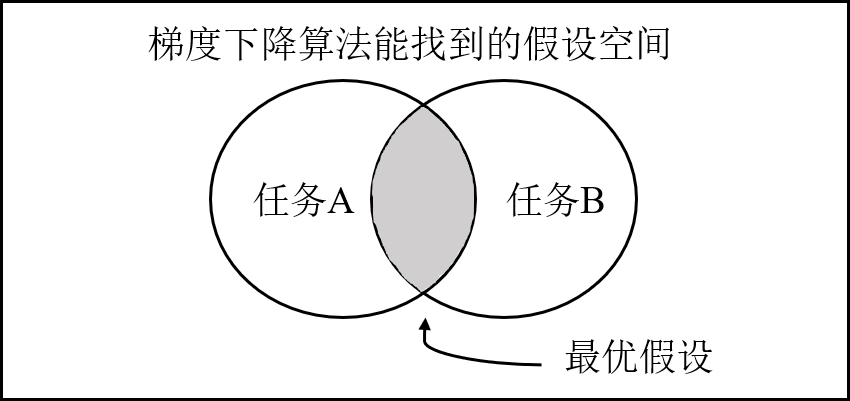
\includegraphics[scale=0.55]{mtl_int.png}
	\caption{多任务学习的一种直观解释}
	\label{fig:mtl_int}
\end{figure}

关于多任务学习为何有效,除了上面的解释(归纳偏置)之外,Caruana还给出了几种合理的解释\cite{Caruana1997}:

\begin{itemize}
	\item \textbf{数据增强(Statistical data amplification)} 由于多个任务的数据集通常是不同的,使用多个相关任务对同一个模型进行训练相当于增大了训练数据量。
	\item \textbf{特征选择(Attribute selection)} 如果任务噪声较大,或者数据高维而数据量有限,模型很难分辨相关特征和无关特征,而多任务学习可以帮助模型选出相关特征,因为这些特征通常在多个任务中是共用的。也就是说,其他任务为模型选择特征提供了额外的证据。
	\item \textbf{窃听(Eavesdropping)} 存在某些特征对于任务 $A$ 易于学习,而对于任务 $B$ 则难以学习。通过多任务学习,模型可以在执行任务 $B$ 时使用任务 $A$ 学到的特征。
\end{itemize}

在深度学习之前,多任务学习已经被应用在线性模型、核方法、决策树、多层感知机等传统机器学习算法上,有大量的研究集中在稀疏正则化\cite{DBLP:conf/nips/ArgyriouEP06}\cite{DBLP:conf/colt/LouniciPTG09}以及学习任务之间的关系\cite{DBLP:journals/jmlr/EvgeniouMP05}\cite{DBLP:conf/nips/JacobBV08}上。

随着深度学习的发展,多任务学习开始应用在深层神经网络中,并在自然语言处理\cite{DBLP:conf/icml/CollobertW08}、计算机视觉\cite{DBLP:conf/cvpr/MisraSGH16}、语音识别\cite{DBLP:conf/icassp/DengHK13}、药物设计\cite{DBLP:journals/corr/RamsundarKRWKP15}等众多应用场景中取得了成功。同时,多任务学习作为一种模型无关的方法,在卷积神经网络\cite{DBLP:conf/icml/CollobertW08}\cite{DBLP:conf/cvpr/MisraSGH16}、循环神经网络\cite{DBLP:conf/ijcai/LiuQH16}、图网络\cite{liu2018multi}上都可以应用。

然而,无论是在传统机器学习算法上还是在深层神经网络上,多任务学习的核心观点都在于知识共享。如何为特定任务和学习算法设计合适的共享模式一直是多任务学习的重要问题。从多任务学习的应用方式来看,可以大概分为下面四种共享模式:

\begin{itemize}
	\item \textbf{硬共享模式}:为多个任务联合训练单个模型,让不同任务共享相同的神经网络层来提取任务无关的通用特征表示,每个任务通过自己的任务特定层在通用表示基础上进行加工得到任务特定表示。
	\item \textbf{软共享模式}:为每个任务训练自己的模型,但每个任务都可以窃听其他任务的模型学习到的特征表示。窃听的方式可以是注意力机制、门控机制,也可以是简单的线性加权。
	\item \textbf{分层共享模式}:为多个任务联合训练单个模型,但简单任务在神经网络低层施加监督信号,困难任务在神经网络的高层施加监督信号。
	\item \textbf{共享-私有模式}:为每个任务训练单个模型,同时使用多个任务训练一个共享模型。每个任务的模型在提取自己任务特定表示的时候也可以从共享模型中提取任务无关的通用特征。
\end{itemize}
四种共享模式如图~\ref{fig:mtl_archs}~所示,图中灰色模块为共享层。关于基于神经网络的多任务学习共享模式的类型,有的文献\cite{ruder2017overview}\cite{DBLP:conf/iclr/MeyersonM18}有不同的分类方式,但硬共享和软共享是两种公认的模式。

\begin{figure}[htb]
	\centering
	
	\subfloat[硬共享模式]{
		\centering
		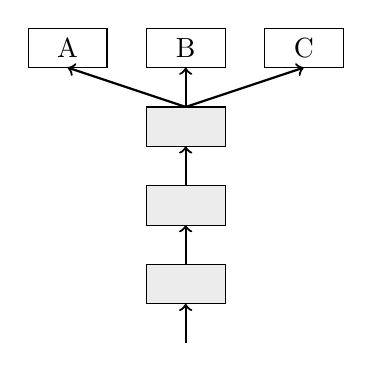
\begin{tikzpicture}
		\begin{scope} [fill opacity = .3]
		\draw [->, thick] (0,0) -- (0, 0.5);
		\draw [fill=lightgray, draw = black] (-0.5,1) rectangle (0.5, 0.5);
		\draw [->, thick] (0, 1) -- (0, 1.5);
		\draw [fill=lightgray, draw = black] (-0.5,2) rectangle (0.5, 1.5);
		\draw [->, thick] (0, 2) -- (0, 2.5);
		\draw [fill=lightgray, draw = black] (-0.5,3) rectangle (0.5, 2.5);
		\draw [draw = black] (-2,4) rectangle (-1, 3.5);
		\draw [draw = black] (-0.5,4) rectangle (0.5, 3.5);
		\draw [draw = black] (1,4) rectangle (2, 3.5);
		\draw [->, thick] (0, 3) -- (-1.5, 3.5);
		\draw [->, thick] (0, 3) -- (0, 3.5);
		\draw [->, thick] (0, 3) -- (1.5, 3.5);
		\end{scope}
		\node at (-1.5, 3.75) {A};
		\node at (0, 3.75) {B};
		\node at (1.5, 3.75) {C};
		
		\end{tikzpicture}
	}
	\hspace{.5in}
	\subfloat[软共享模式]{
		\centering
		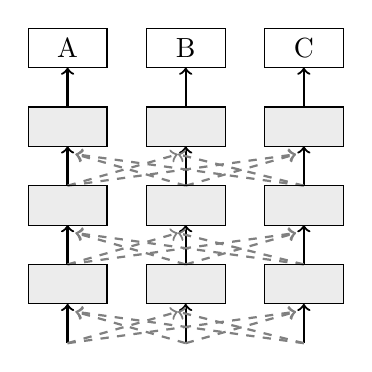
\begin{tikzpicture}
		\begin{scope} [fill opacity = .3]
		\draw [->, thick] (-1.5,0) -- (-1.5, 0.5);
		\draw [->, thick, gray, dashed] (-1.5,0) -- (-.1, 0.4);
		\draw [->, thick, gray, dashed] (-1.5,0) -- (1.4, 0.4);
		
		\draw [->, thick] (-1.5, 1) -- (-1.5, 1.5);
		\draw [->, thick, gray, dashed] (-1.5, 1) -- (-.1, 1.4);
		\draw [->, thick, gray, dashed] (-1.5, 1) -- (1.4, 1.4);
		
		\draw [->, thick] (-1.5, 2) -- (-1.5, 2.5);
		\draw [->, thick, gray, dashed] (-1.5, 2) -- (-.1, 2.4);
		\draw [->, thick, gray, dashed] (-1.5, 2) -- (1.4, 2.4);
		
		\draw [->, thick] (-1.5, 3) -- (-1.5, 3.5);
		
		\draw [fill=lightgray, draw = black] (-2,1) rectangle (-1, 0.5);
		\draw [fill=lightgray, draw = black] (-2,2) rectangle (-1, 1.5);
		\draw [fill=lightgray, draw = black] (-2,3) rectangle (-1, 2.5);
		\draw [draw = black] (-2,4) rectangle (-1, 3.5);
		
		\draw [->, thick] (0,0) -- (0, 0.5);
		\draw [->, thick, gray, dashed] (0,0) -- (-1.4, 0.4);
		\draw [->, thick, gray, dashed] (0,0) -- (1.4, 0.4);
		
		\draw [->, thick] (0, 1) -- (0, 1.5);
		\draw [->, thick, gray, dashed] (0, 1) -- (-1.4, 1.4);
		\draw [->, thick, gray, dashed] (0, 1) -- (1.4, 1.4);
		
		\draw [->, thick] (0, 2) -- (0, 2.5);
		\draw [->, thick, gray, dashed] (0, 2) -- (-1.4, 2.4);
		\draw [->, thick, gray, dashed] (0, 2) -- (1.4, 2.4);
		
		\draw [->, thick] (0, 3) -- (0, 3.5);
		
		\draw [fill=lightgray, draw = black] (-0.5,1) rectangle (0.5, 0.5);
		\draw [fill=lightgray, draw = black] (-0.5,2) rectangle (0.5, 1.5);
		\draw [fill=lightgray, draw = black] (-0.5,3) rectangle (0.5, 2.5);
		\draw [draw = black] (-0.5,4) rectangle (0.5, 3.5);
		
		\draw [->, thick] (1.5, 0) -- (1.5, 0.5);
		\draw [->, thick, gray, dashed] (1.5, 0) -- (-1.4, 0.4);
		\draw [->, thick, gray, dashed] (1.5, 0) -- (-.1, 0.4);
		
		\draw [->, thick] (1.5, 1) -- (1.5, 1.5);
		\draw [->, thick, gray, dashed] (1.5, 1) -- (-1.4, 1.4);
		\draw [->, thick, gray, dashed] (1.5, 1) -- (-.1, 1.4);
		
		\draw [->, thick] (1.5, 2) -- (1.5, 2.5);
		\draw [->, thick, gray, dashed] (1.5, 2) -- (-1.4, 2.4);
		\draw [->, thick, gray, dashed] (1.5, 2) -- (-.1, 2.4);
		
		\draw [->, thick] (1.5, 3) -- (1.5, 3.5);
		
		\draw [fill=lightgray, draw = black] (1,1) rectangle (2, 0.5);
		\draw [fill=lightgray, draw = black] (1,2) rectangle (2, 1.5);
		\draw [fill=lightgray, draw = black] (1,3) rectangle (2, 2.5);
		\draw [ draw = black] (1,4) rectangle (2, 3.5);
		\end{scope}
		\node at (-1.5, 3.75) {A};
		\node at (0, 3.75) {B};
		\node at (1.5, 3.75) {C};
		
		\end{tikzpicture}
	}
	\vspace{.2in}
	
	\subfloat[分层共享模式]{
		\centering
		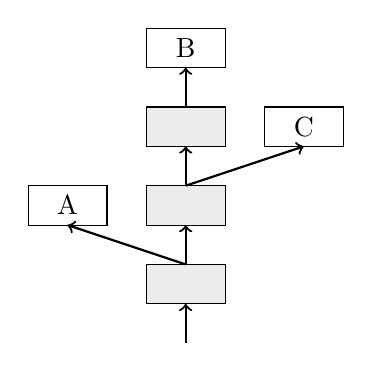
\begin{tikzpicture}
		\begin{scope} [fill opacity = .3]
		\draw [->, thick] (0,0) -- (0, 0.5);
		\draw [->, thick] (0, 1) -- (0, 1.5);
		\draw [->, thick] (0, 2) -- (0, 2.5);
		\draw [->, thick] (0, 3) -- (0, 3.5);
		\draw [->, thick] (0, 1) -- (-1.5, 1.5);
		\draw [->, thick] (0, 2) -- (1.5, 2.5);
		
		\draw [fill=lightgray, draw = black] (-0.5,1) rectangle (0.5, 0.5);
		\draw [fill=lightgray, draw = black] (-0.5,2) rectangle (0.5, 1.5);
		\draw [fill=lightgray, draw = black] (-0.5,3) rectangle (0.5, 2.5);
		
		\draw [ draw = black] (-0.5,4) rectangle (0.5, 3.5);
		\draw [ draw = black] (-2,2) rectangle (-1, 1.5);
		\draw [ draw = black] (1,3) rectangle (2, 2.5);
		\end{scope}
		\node at (-1.5, 1.75) {A};
		\node at (0, 3.75) {B};
		\node at (1.5, 2.75) {C};
		
		\end{tikzpicture}
	}
	\hspace{.5in}
	\subfloat[共享-私有模式]{
		\centering
		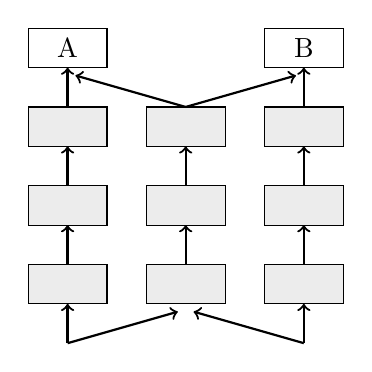
\begin{tikzpicture}
		\begin{scope} [fill opacity = .3]
		\draw [->, thick] (-1.5,0) -- (-1.5, 0.5);
		\draw [->, thick] (-1.5, 1) -- (-1.5, 1.5);
		\draw [->, thick] (-1.5, 2) -- (-1.5, 2.5);
		\draw [->, thick] (-1.5, 3) -- (-1.5, 3.5);
		
		\draw [fill=lightgray, draw = black] (-2,1) rectangle (-1, 0.5);
		\draw [fill=lightgray, draw = black] (-2,2) rectangle (-1, 1.5);
		\draw [fill=lightgray, draw = black] (-2,3) rectangle (-1, 2.5);
		\draw [ draw = black] (-2,4) rectangle (-1, 3.5);
		
		\draw [->, thick] (-1.5,0) -- (-.1, .4);
		\draw [->, thick] (1.5,0) -- (.1, .4);
		\draw [->, thick] (0, 1) -- (0, 1.5);
		\draw [->, thick] (0, 2) -- (0, 2.5);
		\draw [->, thick] (0, 3) -- (-1.4, 3.4);
		\draw [->, thick] (0, 3) -- (1.4, 3.4);
		
		\draw [fill=lightgray, draw = black] (-0.5,1) rectangle (0.5, 0.5);
		\draw [fill=lightgray, draw = black] (-0.5,2) rectangle (0.5, 1.5);
		\draw [fill=lightgray, draw = black] (-0.5,3) rectangle (0.5, 2.5);
		
		\draw [->, thick] (1.5, 0) -- (1.5, 0.5);
		\draw [->, thick] (1.5, 1) -- (1.5, 1.5);
		\draw [->, thick] (1.5, 2) -- (1.5, 2.5);
		\draw [->, thick] (1.5, 3) -- (1.5, 3.5);
		
		\draw [fill=lightgray, draw = black] (1,1) rectangle (2, 0.5);
		\draw [fill=lightgray, draw = black] (1,2) rectangle (2, 1.5);
		\draw [fill=lightgray, draw = black] (1,3) rectangle (2, 2.5);
		\draw [ draw = black] (1,4) rectangle (2, 3.5);
		\end{scope}
		\node at (-1.5, 3.75) {A};
		\node at (1.5, 3.75) {B};
		
		\end{tikzpicture}
	}
	\caption{多任务学习的几种常见共享模式}
	\label{fig:mtl_archs}
\end{figure}

具体的,我们以最常见的硬共享模式为例,给出多任务学习的形式化描述。假设有~$T$~个相关任务,任务~$t$~的数据集为~$\mathcal{D}_t = \lbrace \mathbf{x}_n^{(t)}, y_n^{(t)} \rbrace_{n=1}^{N_t}$,包含~$N_t$~个样本。假设模型在任务~$t$~的第~$n$~个样本上的输出为
\begin{equation}
	\hat{y}_n^{(t)} = \mathcal{G}^{(t)}(\mathcal{F}(\mathbf{x}_n^{(t)}; \theta_\mathcal{F}) ; \theta_{\mathcal{G}^{(t)}}),
\end{equation}
其中~$\mathcal{F}$~为神经网络共享层,$\mathcal{G}^{(t)}$~为任务~$t$~的特定层。模型总参数包含共享层的参数以及任务特定层的参数,即~$\theta = [\theta_\mathcal{F}, \{ \theta_{\mathcal{G}^{(t)}}\}_{t=1}^T]$. 多任务联合学习的损失函数为
\begin{equation}
	\mathcal{L}(\theta) = \sum_{t=1}^T\lambda_t\sum_{n=1}^{N_t}\mathcal{L}_t(\hat{y}_n^{(t)}, y_n^{(t)}),
\end{equation}
其中,$\mathcal{L}_t(\cdot)$~为第~$t$~个任务的损失函数,$\lambda_t$~为第~$t$~个任务损失函数的权重。$\lambda_t$~通常被看作是超参数,根据任务~$t$~的重要程度或困难程度来确定,也可以作为可学习参数根据任务的不确定性来自主学习\cite{DBLP:conf/cvpr/KendallGC18}。

最后,通过优化如下目标来得到模型参数
\begin{equation}
	\theta ^* = \mathop{\arg\min}\limits_{\theta} \mathcal{L}(\theta).
\end{equation}
多任务学习使用的优化算法与常见单任务学习的优化算法没有什么不同,可以采用随机梯度下降等方法。
\section{自然语言处理}
\label{sec:nlp}

\emph{自然语言处理}(Natural Language Processing, NLP)是一门涵盖计算机科学、语言学、数学等多个领域的交叉学科,也是人工智能的核心领域之一,旨在使用计算机技术来处理、理解和生成自然语言文本。同时,自然语言处理也是一个包括词性标注、句法分析、语义角色分析、机器翻译、阅读理解、问答系统、对话系统等在内的庞大的研究领域。从定义上,任何与处理文本数据相关的问题都可以归为自然语言处理的问题。

事实上,人们对NLP的研究早在人工智能被提出之前就开始了。上世纪上半叶,Claude Shannon使用概率模型来描述人类语言,提出用熵来表示语言的不确定性。1956年,Noam Chomsky提出生成语法理论,给出了语言句法结构的符号规则,此后,基于规则的符号系统开始在NLP领域流行。研究人员根据研究工具的不同分为统计和规则两个流派。到上世纪末,随着隐马尔科夫模型、核方法等方法的出现,统计自然语言处理开始因其灵活性和通用性渐渐成为主流。随着深度学习的兴起,这一趋势被再次加强,基于神经网络的方法开始在各大NLP任务上取得~\sArt~结果。

在深度学习背景下,一个使得NLP取得重大进展的关键概念是\emph{分布式表示}(Distributed Representation)\cite{Hinton:1986:DR:104279.104287}。在传统机器学习方法中,普遍采用one-hot方法表示文本特征,即在一向量中用1来表示出现的单词,用0来表示未出现的单词。然而这种表示方法下向量维度与词表大小一致,不便于扩展,且任意两单词之间正交,无法计算语义相似度。而分布式表示则将文本语义分布到向量的各个维度,或者说分布到多个神经元上进行处理。在分布式表示下,文本用低维稠密向量表示,使得语义组合和语义相似度的计算都非常灵活。分布式表示的概念是整个深度学习技术的核心,如何学到一个好的分布式表示是决定各个深度学习算法性能的关键。

在NLP中,文本的分布式表示方法一直是研究重点。分布式表示的应用引出了\emph{词向量}(也被称作\emph{词嵌入})的概念,在词嵌入矩阵中,每个单词用一个低维稠密词向量来表示。最初,Bengio等人\cite{DBLP:conf/nips/BengioDV00}将分布式表示引入语言建模,让神经网络在反向传播时同时更新网络参数和词向量。这里的词向量作为模型的参数,训练前采用随机初始化。2013年,Mikolov等人\cite{DBLP:conf/nips/MikolovSCCD13}提出了word2vec方法,可以在大规模无标注文本上预训练一组词向量,使用预训练的词向量初始化神经网络的词嵌入层可以显著提升模型效果。2014年,Pennington等人\cite{DBLP:conf/emnlp/PenningtonSM14}使用类似的思路发明了GloVe,这种词向量具备更好的线性性质。从此,在绝大多数NLP任务中,人们通常使用预训练好的词向量来作为模型输入,而不再是随机初始化。然而,这些文本表示方法将单词映射为固定的词向量,难以处理一词多义的问题,因此是\emph{未语境化}(non-contextualized)的。在现实场景中,一个词的意思常常要通过其所在的语境来确定,例如“苹果”在某些语境中表示一种水果,而在某些语境中可能表示一家公司。为处理这一问题,人们提出了\emph{语境化}(contextual)的文本表示方法,如ELMo\cite{DBLP:conf/naacl/PetersNIGCLZ18},GPT\cite{radford2018improving},BERT\cite{devlin2018bert}等,这些上下文敏感的文本表示方法使得神经网络模型在各大NLP任务上取得了巨大的提升。

文本的分布式表示一般被认为是神经网络的输入,即第一层(词嵌入层)。为执行特定的任务,通常需要在文本表示的基础上再进行加工得到易于预测的任务特定表示。这种加工可以采用不同的神经网络来实现。在NLP中,目前普遍使用的神经网络为卷积神经网络(CNN)\cite{DBLP:conf/icml/CollobertW08}\cite{DBLP:conf/emnlp/Kim14}\cite{DBLP:conf/icml/GehringAGYD17}和循环神经网络(RNN)\cite{DBLP:conf/interspeech/MikolovKBCK10}\cite{DBLP:conf/emnlp/WenGMSVY15}\cite{DBLP:conf/acl/MaH16}。然而,这二者还都存在难以解决的缺陷:CNN一般只能建模局部位置信息,难以捕捉长距离句子依赖;而RNN每一时间步的计算都依赖上一时间步的状态,导致其运算速度缓慢,难以并行,无法在大规模工业场景中使用。需要注意的是,本文提到的RNN包含原始版本及其变种,如LSTM\cite{DBLP:journals/neco/GersSC00}和GRU\cite{DBLP:journals/corr/ChungGCB14}.

另外,人们在对自然语言处理、计算机视觉等问题的研究过程中也提出了一些模型无关的机制,其中的一个典型代表就是\emph{注意力机制}。在NLP中,注意力机制最初出现在机器翻译中,显著提升了翻译质量\cite{DBLP:journals/corr/BahdanauCB14}。随后,注意力机制开始在NLP的各个子问题中被广泛使用,基于双向LSTM和注意力机制的神经网络模型一度成为处理包括阅读理解、自然语言推理等在内的各个NLP任务的标配。甚至在2017年,Google提出了完全基于自注意力的神经网络:Transformer\cite{DBLP:conf/nips/VaswaniSPUJGKP17},在机器翻译任务上取得了新的~\sArt~结果。

%\begin{figure}[htb]
%	\centering
%	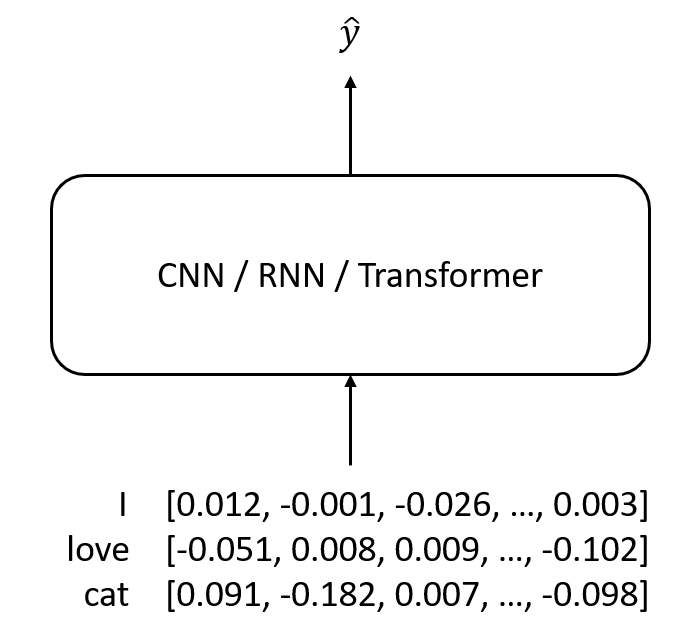
\includegraphics[scale=0.6]{nlp_ppl.png}
%	\caption{基于神经网络处理自然语言的一般模式}
%	\label{fig:nlp_ppl}
%\end{figure}

Transformer在语义信息提取和长距离依赖任务上都取得了富有竞争力的结果\cite{DBLP:conf/emnlp/TangMRS18},并且因其可以并行计算的优点在NLP领域迅速流行。近期,随着基于Transformer的预训练模型BERT\cite{devlin2018bert}取得的巨大成功,Transformer开始受到越来越多的研究者关注,出现了Universal Transformer\cite{dehghani2018universal}、Gaussian Transformer\cite{guo2019gaussian}、Star-Transformer\cite{guo2019star}等变种。

%图~\ref{fig:nlp_ppl}~比较简略地给出了文本从输入神经网络到输出的一般模式。

\section{神经多任务自然语言处理}
\label{sec:mtl4nlp}
在前文中,介绍了深度学习的基本概念,以及多任务学习和自然语言处理在深度学习背景下的研究现状。在这一基础上,本节将介绍使用基于神经网络的多任务学习在自然语言处理中的主要进展。

事实上,早在十年前就已经有人在神经网络模型中应用多任务学习来解决NLP的问题:Collobert等人\cite{DBLP:conf/icml/CollobertW08}使用一个简单的卷积神经网络(Convolutional Neural Network, CNN)来同时学习词性标注、语块标注、命名实体识别、语义角色标注、语义相似度和语言模型,超越了CNN使用单任务训练时的表现。

随着循环神经网络(Recurrent Neural Network, RNN)在NLP上的广泛应用,研究者开始基于RNN构造多任务学习框架,在机器翻译\cite{DBLP:conf/acl/DongWHYW15}、文本分类\cite{DBLP:conf/ijcai/LiuQH16}\cite{DBLP:conf/acl/LiuQH17}、序列标注\cite{DBLP:conf/acl/SogaardG16}等常见NLP任务上均取得了成功。

图~\ref{fig:mtl_cnn_rnn}~分别给出了多任务学习在CNN和RNN上的两种模型结构:(a) 使用多任务CNN处理词性标注、命名实体识别等多个序列标注任务和语义相似度任务;(b) 使用多任务RNN处理多语言机器翻译问题。两模型均属于多任务学习中的硬共享结构,且(a)模型仅共享词表。

\begin{figure}[htb]
	\centering
	\subfloat[一种多任务CNN模型\cite{DBLP:conf/icml/CollobertW08}]{
		\centering
		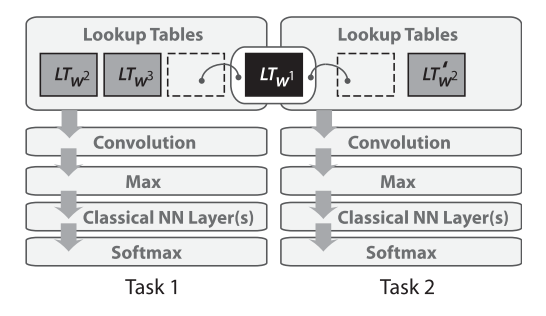
\includegraphics[scale=0.55]{MTL-CNN.PNG}
	}
	\subfloat[一种多任务RNN模型\cite{DBLP:conf/acl/DongWHYW15}]{
		\centering
		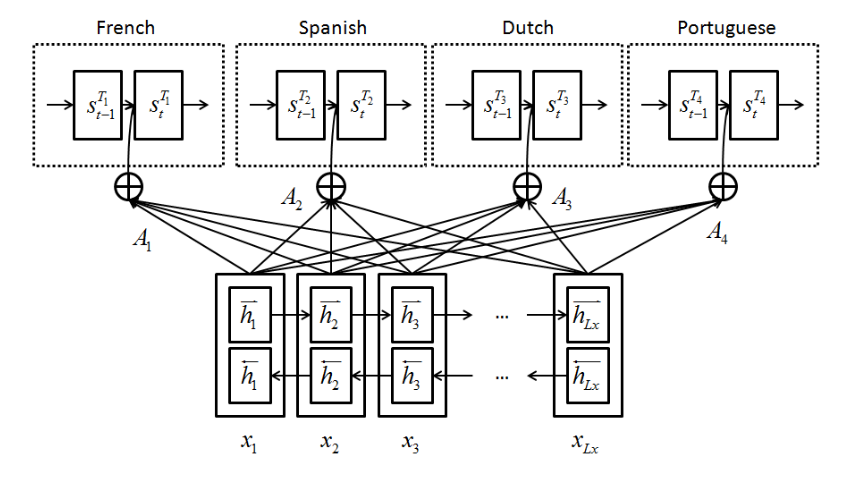
\includegraphics[scale=0.45]{MTL-RNN.PNG}
	}
	\caption{多任务学习在CNN和RNN上的应用示例}
	\label{fig:mtl_cnn_rnn}
\end{figure}

从共享架构上看,基于神经网络的多任务学习架构涵盖了前文提到的各种共享模式。首先,最简单的硬共享模式率先得到了应用\cite{DBLP:conf/icml/CollobertW08},并且直到今天还在被广泛的使用\cite{liu2019multi};随后,软共享模式因其灵活性也被广泛地应用在NLP任务中,并取得了出色的表现\cite{1705.08142};由于NLP任务对文本表示的要求不同(例如比较简单的NLP任务仅需要简单的语法知识而难度较大的任务需要复杂的语义信息),分层共享在RNN中得到了应用\cite{DBLP:conf/acl/SogaardG16},取得了优于硬共享架构的效果;最后,Liu等人\cite{DBLP:conf/ijcai/LiuQH16}在RNN中使用共享-私有模式,在文本分类任务上取得了较大提升。

近期,随着迁移学习在NLP领域取得了巨大成功\cite{DBLP:conf/naacl/PetersNIGCLZ18}\cite{radford2018improving}\cite{devlin2018bert},人们发现学习一个通用的任务无关的表示能够给特定任务带来的收益远远大于根据任务特点对模型结构的改进。为了评测模型的通用表示能力,研究者们开始使用多个任务的性能来测试单一模型,开发了通用表示能力评测工具(SentEval\cite{DBLP:conf/lrec/ConneauK18})以及一些多任务基准平台(DecaNLP\cite{mccann2018natural}、GLUE\cite{DBLP:conf/emnlp/WangSMHLB18})。

2018年10月,BERT\cite{devlin2018bert},一个预训练的Transformer模型,在GLUE的多个任务上的表现都大幅度超越了之前的模型。最近,人们发现在BERT的基础上使用多任务学习对模型进行微调能够取得进一步提升\cite{liu2019multi}\cite{anonymous2018bam!}。

然而,目前还很少有工作在Transformer上探索多任务学习的使用。随着Transformer在机器翻译\cite{DBLP:conf/nips/VaswaniSPUJGKP17}、迁移学习\cite{radford2018improving}\cite{devlin2018bert}中取得了巨大成功,如何使其通过多任务学习取得额外的收益,以及如何对其设计新的共享模式都是值得探索的问题。